% Any part of the report that relates to the basic features.
\section{Basic Features}
\subsection{BVH performance test}
Text Text Text...
\subsection{Light transparency sampling}
The algorithm suffers from two main problems. Firstly, in a scenario where an opaque object directly obstructs, no light is computed even if reflective surfaces around produce incident secondary rays. Secondly, only the obstruction of thin boundary surfaces contributes to the computation, with no consideration to obstructing object's internal medium.
\subsection{Depth of field}
Description:
The method iterates through all the pixels on the screen and calculates the position of the focal point relative to each pixel. It then generates several rays that start from a random location inside the pixel and end at the focal point. It calculates the color that results from the rays and averages their sum, which will be the final color of the pixel.

Visual debug:
There are three sliders in the depth of field section of the GUI: focal length, lens size, and number of samples. Focal length adjusts the distance from the camera to the focal point. Lens size modifies the maximum offset from the center of each pixel to the starting position of each ray. The number of samples specifies how many rays should be generated.

Location:
The method that implements depth of field is called renderImageWithDepthOfField and is located in the extra.cpp file. The only other changes related to this feature were made in main.cpp and common.h for the sliders in the GUI.


\includegraphics[]{Report - Group 100\\rsc\\dof_render1.png}

\includegraphics[]{Report - Group 100\\rsc\\dof_render2.png}
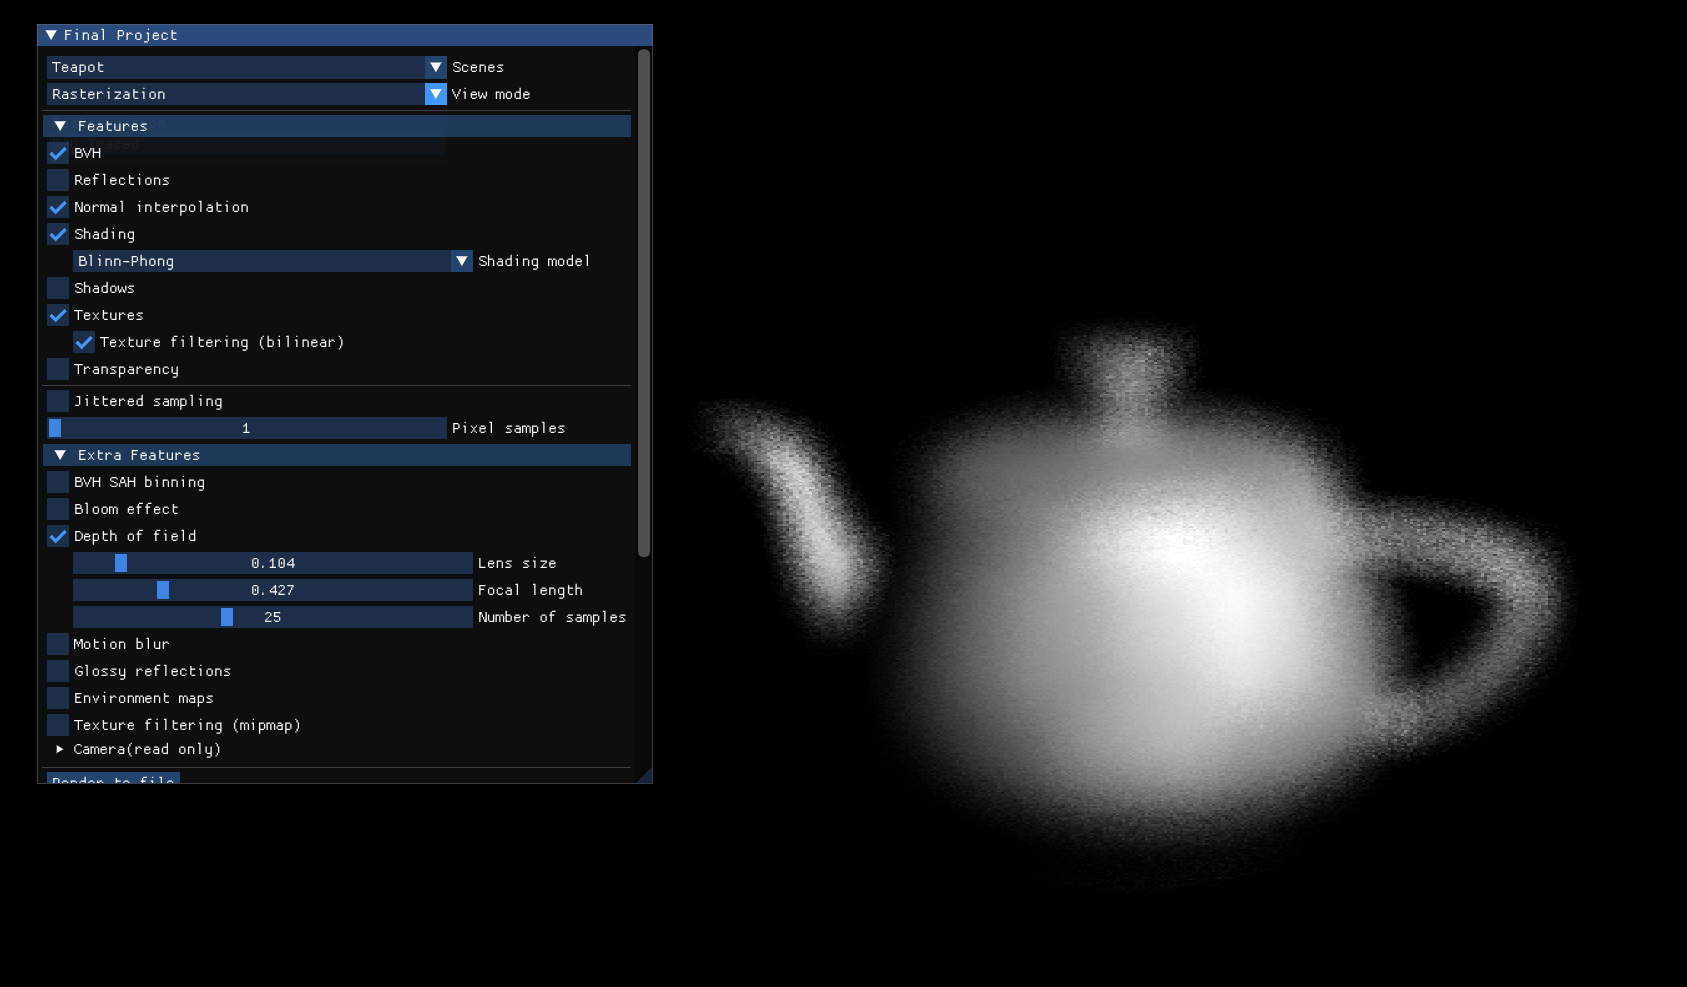
\includegraphics[]{Report - Group 100\\rsc\\dof_render3.png}